\bookchapter{Capitolo 49: Preparare l'ambiente di sviluppo — Android Studio e il primo progetto}

\chapterintro{Chi vuole lavorare bene deve prima affilare gli strumenti. In questo capitolo allestiamo la «cucina»: installiamo Android Studio, facciamo girare l'emulatore, creiamo il primo progetto Android della tua vita e poi smontiamo la struttura del progetto per capire ogni pezzo. Con l'ambiente pronto, vedrai per la prima volta il codice scritto da te trasformarsi in un pulsante che si può toccare — un momento che a molti resta in cuore per tutta la vita.}

\booksection{Installare Android Studio}

Android Studio è l'ambiente di sviluppo integrato (IDE) ufficiale di Google: è gratuito e ha tutto a bordo — scrivere codice, vedere l'anteprima dell'interfaccia, fare debug, creare i pacchetti. Installazione in quattro passi:

\begin{enumerate}
  \item Apri il sito ufficiale developer.android.com/studio e scarica l'ultima versione stabile (ad agosto 2026 la versione successiva a Narwhal, disponibile per Windows/Mac/Linux);
  \item Avvia il pacchetto d'installazione e vai sempre avanti con «Avanti» — l'assistente includerà in automatico l'Android SDK e i componenti dell'emulatore;
  \item Al primo avvio scarica i componenti dell'SDK come indicato (va bene lasciare le spunte predefinite: servono qualche minuto e qualche GB di spazio);
  \item Finito, vedrai la pagina di benvenuto — complimenti, la «cucina» è pronta.
\end{enumerate}

\begin{tcbwarn}{Attenzione: tieni a mente i requisiti hardware}
Android Studio è un tipo che «mangia memoria»: si consigliano almeno 16 GB di RAM (con 8 GB funziona, ma l'emulatore tende a scattare), 20 GB o più di disco libero e una CPU con supporto alla virtualizzazione (attiva VT-x/AMD-V nel BIOS). Se il computer è davvero datato, puoi sostituire l'emulatore con il «debug su dispositivo reale» (ne parliamo nella sezione 4 di questo capitolo): l'esperienza è persino più fluida.

\end{tcbwarn}

\booksection{Creare il tuo primo progetto}

Nella pagina di benvenuto clicca su New Project, scegli il modello Empty Activity (il più pulito per chi inizia) e compila tre cose:

\begin{center}
\begin{tabularx}{\linewidth}{|X|X|X|}
\hline
\textbf{Voce di configurazione} & \textbf{Cosa inserire} & \textbf{Spiegazione} \tabularnewline
\hline
Name & My First App & Nome dell'app, quello che appare nella schermata home del telefono \tabularnewline
Package name & com.example.myfirstapp & Identificativo univoco in tutto il mondo; per convenzione si usa il «dominio invertito», per ora lascia quello proposto \tabularnewline
Minimum SDK & API 26(Android 8.0) & Versione minima supportata: così copri il 95\% e più dei dispositivi \tabularnewline
\hline
\end{tabularx}
\end{center}

\begin{center}\small\color{gray}Le tre cose da compilare per creare un progetto\end{center}

Dopo Finish, Android Studio con Gradle scaricherà in automatico le dipendenze e compilerà il progetto (la prima volta aspetta qualche minuto, poi ogni volta sarà molto più rapido). A build finita hai un'app che si può avviare — anche se per ora sa solo mostrare una riga: “Hello Android!”.

\begin{tcbinfo}{Consiglio: i segreti del nome del pacchetto}
Il nome del pacchetto (package name) è come la «carta d'identità» dell'app: non può ripetersi in tutto il mondo e, una volta pubblicata l'app, non si può più cambiare. Per gli esercizi personali basta com.example.xxx; per un prodotto vero serve il tuo dominio invertito (per esempio com.tuonome.app). Non pubblicare con com.example — lo store la respinge.

\end{tcbinfo}

\booksection{Farlo girare: emulatore e dispositivo reale}

Il codice è pronto: serve un «telefono» su cui farlo girare. Hai due possibilità:

\booksubsection{L'emulatore (Emulator)}

L'emulatore crea un telefono Android virtuale dentro il computer. In Android Studio apri Device Manager Create Device, scegli un dispositivo (consigliata la serie Pixel) seleziona un'immagine di sistema (quella con le Google APIs) scaricala avviala. Poi clicca sul triangolo verde Run nella barra degli strumenti: dopo pochi secondi la tua app compare sullo schermo del «telefono».

\booksubsection{Il debug su dispositivo reale (più consigliato)}

Il dispositivo reale resta l'ambiente di prova più fedele — la sensazione degli scorrimenti, la rete vera, i sensori veri: l'emulatore non gli si avvicina. E il debug su un telefono Android vero è semplicissimo:

\begin{enumerate}
  \item Sul telefono apri [Impostazioni] [Info sul telefono], tocca 7 volte di fila «Numero build» per attivare le «Opzioni sviluppatore»;
  \item In [Opzioni sviluppatore] attiva il Debug USB;
  \item Collega il telefono al computer con il cavo dati e nel popup del telefono scegli «Consenti debug USB»;
  \item Torna in Android Studio: il tuo telefono comparirà nel menu a tendina dei dispositivi in alto; clicca Run.
\end{enumerate}

\textbf{Attenzione alle trappole: non tenere il debug USB sempre attivo}\par

Il debug USB equivale ad aprire al computer una «porta sul retro». Quando carichi il telefono in luoghi pubblici o lo colleghi a computer di cui non ti fidi, chiudi sempre il debug USB, così nessuno potrà leggere i tuoi dati da lì. Quando hai finito di sviluppare, spegnilo: prendine l'abitudine.

\booksection{Anatomia del progetto: a cosa serve ogni file}

La prima volta che apri il progetto, l'albero dei file a sinistra può girarti la testa. Niente panico: nel lavoro di tutti i giorni il 90\% del tempo avrai a che fare solo con questi:

\begin{center}
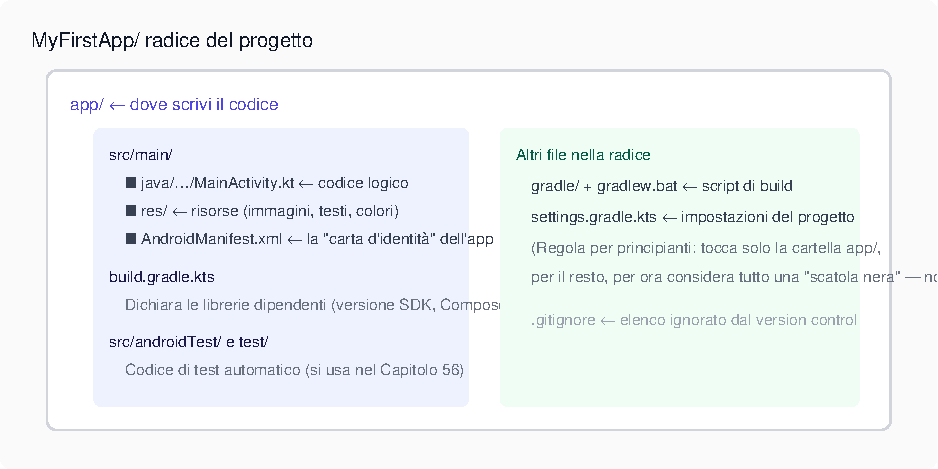
\includegraphics[width=0.92\linewidth]{figures/fig-di-si-shi-jiu-zhang-1}
\\[2pt]\small Figura 2: la struttura del progetto che un principiante deve conoscere (regola pratica: tocca solo la cartella app/)
\end{center}

\begin{itemize}
  \item MainActivity.kt: la «porta d'ingresso» dell'app. Quando l'utente tocca l'icona, è la prima cosa che si sveglia. Nel modello attuale si occupa di mostrare "Hello Android!".
  \item AndroidManifest.xml: la «carta d'identità» dell'app — dichiara come si chiama l'app, quale icona usa, quali schermate ha e quali permessi richiede (fotocamera, posizione, ecc.).
  \item Cartella res/: il magazzino delle risorse, dove stanno immagini, icone, testi e colori. Mettere i testi nei file di risorse invece di scriverli fissi nel codice è una buona abitudine dello sviluppo Android (comodissimo per cambiare lingua o tema).
  \item build.gradle.kts: la «ricetta» della build — dichiara la versione minima supportata e da quali librerie dipende il progetto (per esempio Compose).
\end{itemize}

\booksection{Primo colpo di mano: cambia “Hello” con il tuo nome}

Apri MainActivity.kt: vedrai il codice generato dal modello Compose. Trova la riga Text(“Hello Android!”), sostituisci il testo tra virgolette con il tuo nome, per esempio Text(“Ciao, sono Maria! Questa è la mia prima app”), poi premi Ctrl+R (Cmd+R su Mac) per rilanciare. Dopo qualche secondo, sull'emulatore comparirà il tuo nome.

\begin{lstlisting}[language=Kotlin]
setContent {
    MyFirstAppTheme {
        Surface(modifier = Modifier.fillMaxSize()) {
            // v cambia questo testo con il tuo
            Text("Ciao, Marco! Questa è la mia prima app")
        }
    }
}
\end{lstlisting}

Congratulazioni: hai appena completato un intero ciclo «modifico il codice compilo installo eseguo». Questo ciclo è la routine di sviluppo di ogni giorno a venire. Già che sei in calore, prova a cambiare qualcos'altro: aumenta la dimensione del testo, cambia colore — nel prossimo capitolo scopriremo da dove nascono queste «magie».

\booksection{Pronto soccorso degli errori comuni: la «sala d'emergenza» delle prime due settimane da principiante}

Nella fase di preparazione dell'ambiente e di prima build molto probabilmente incontrerai i tre errori qui sotto. Niente panico: hanno tutti la loro cura:

\begin{center}
\begin{tabularx}{\linewidth}{|X|X|X|}
\hline
\textbf{Come si presenta l'errore} & \textbf{Causa tipica} & \textbf{La cura} \tabularnewline
\hline
Gradle sync failed / dipendenze che scaricano lento & Connessione ai repository in rete in difficoltà & Configura per Gradle dei repository mirror (mirror Maven di Alibaba Cloud/Tencent Cloud): cerca online «gradle mirror repository» e segui le istruzioni per modificarlo \tabularnewline
Componenti SDK mancanti & Il download dell'SDK è stato saltato in fase d'installazione & Settings SDK Manager: installare piattaforme e strumenti mancanti \tabularnewline
L'emulatore non parte / schermo nero & Virtualizzazione non attiva, immagine danneggiata & Attiva VT-x/AMD-V nel BIOS; cancella e ricrea l'emulatore; oppure passa direttamente al debug su dispositivo reale \tabularnewline
\hline
\end{tabularx}
\end{center}

\begin{center}\small\color{gray}Tabella di pronto soccorso per gli errori d'ambiente del principiante\end{center}

\begin{tcbinfo}{Consiglio: il metodo per cercare gli errori}
La prima riga del messaggio d'errore è la più preziosa — copiala così com'è nel motore di ricerca, aggiungendo la parola chiave “android studio”. Non cercare domande vaghe tipo «come faccio a installare l'ambiente», ma errori precisi tipo “Gradle sync failed: Could not resolve com.android.tools.build”. Solo le domande precise ottengono risposte precise.

\end{tcbinfo}

\begin{tcbpractice}{Mani all'opera: completa la tua «checklist» di riti da sviluppatore}
(1) Installa Android Studio e fai girare l'emulatore; (2) avvia una volta la tua app su un dispositivo reale e salva uno screenshot come ricordo; (3) cambia il testo Hello con il tuo nome; (4) comprimi il progetto e conservane un archivio. Fatti questi quattro passi, potrai annunciare agli amici: anch'io sono uno sviluppatore Android (screenshot alla mano).

\end{tcbpractice}

\begin{tcbsummary}{Riepilogo del capitolo}
\begin{itemize}
  \item Android Studio = IDE ufficiale e gratuito; consigliati 16 GB di RAM + 20 GB di disco + virtualizzazione attiva
  \item I tre ingredienti di un nuovo progetto: nome, nome del pacchetto (univoco al mondo, niente pubblicazione con com.example), SDK minimo (da API 26)
  \item Due modi di eseguire: l'emulatore (telefono virtuale nel computer) e il dispositivo reale (attiva il debug USB e ricordati di chiuderlo dopo l'uso)
  \item La regola del progetto: tocca solo la cartella app/ — MainActivity.kt è la porta d'ingresso, il Manifest è la carta d'identità, res/ è il magazzino delle risorse
  \item La routine di sviluppo = cambi il codice Run guardi il risultato, e si riparte
\end{itemize}

\end{tcbsummary}
